In the Heat Transfer algorithm~(HT), we have a graph where heat values
are exchanged between nodes. The program stops when the new heat
values of every node are $\delta = |H_i - H_{i-1}| \le \epsilon$. The
algorithm works asynchronously, i.e., heat values are updated using
information as it arrives from neighboring nodes. This increases
parallelism since nodes do not need to synchronize between iterations.

Fig.~\ref{code:ht} shows the HT rules that send new heat values to
neighbor nodes. In the first rule we added \texttt{add-priority} to increase the priority of the neighbor
nodes if the current node has a large $\delta$. The idea is to prioritize the
computation of heat values of nodes (using \texttt{update}) that have a neighbor
that changed significantly. Multiple \texttt{add-priority} facts will
increase the priority of a node so that nodes with multiple large deltas will
have more priority.

\begin{topfig}
\scriptsize\begin{Verbatim}[numbers=left,commandchars=\\\[\]]
new-heat(A, New, Old),
Delta = fabs(New - Old),
Delta > epsilon
   -o {B | !edge(A, B) |
         new-neighbor-heat(B, A, New),
         update(B), \underline[add-priority(B, Delta)]}.

new-heat(A, New, Old)
fabs(New - Old) <= epsilon
   -o {B | !edge(A, B) |
         new-neighbor-heat(B, A, New)}.
\end{Verbatim}
  \scap{code:ht}{Coordination code for the Heat Transfer program. The
      first rule now increases the priority of neighbor nodes.  The
      logic remains the same as before, however bigger
      changes in heat are now propagated faster.}
\end{topfig}
\normalsize

Fig.~\ref{results:ht} presents the scalability results for the regular
and coordinated version. The dataset used is a square grid with an inner square
with high heat nodes. Comparing the coordinated version with the regular
version, with 1 thread there is a 33\% reduction in run time, while
for 16 threads there is a 18\% reduction.

To further improve locality, we have split the second rule to avoid sending
small $\delta$ values if the target node is in another thread
(Fig.~\ref{code:ht_better}). The \textbf{Local-Only/Regular} line
in Fig.~\ref{results:ht} shows that this has the best performance.  However, this
come at the price of increased errors in the computed heat values.

\begin{topfig}
\scriptsize\begin{Verbatim}[numbers=left,commandchars=\\\[\]]
new-heat(A, New, Old)
fabs(New - Old) <= epsilon
\underline[cpu-id(A, B, C)],
\underline[cpu-id(A, A, C)]
   -o {B, W | !edge(A, B) |
         new-neighbor-heat(B, A, New)}.

new-heat(A, New, Old)
fabs(New - Old) <= epsilon,
\underline[cpu-id(A, B, C1)],
\underline[cpu-id(A, A, C2)],
\underline[C1 <> C2]
   -o 1. // nothing is derived
\end{Verbatim}
  \scap{code:ht_better}{To improve locality, we added a third rule to not send small $\delta$
     values if the neighbor is in another thread.}
\end{topfig}
\normalsize

\begin{topfig}
   \begin{center}
      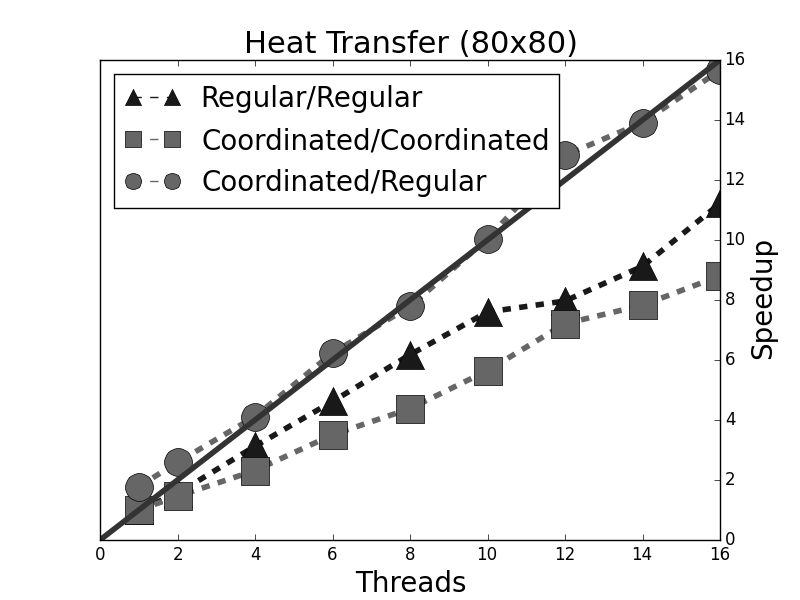
\includegraphics[width=5.5cm]{results/new-heat-transfer-80}
   \end{center}
   \scap{results:ht}{Experimental results for the HT program. The coordinated version
      is, on average, 30\% faster than the regular version although it has a
      slightly worse scalability due to a reduction in work available.}
\end{topfig}
